\chapter{Validación}
\label{sec:validacion}

\begin{quote}
\itshape
Este capítulo describe cómo se validó el sistema: la metodología de prueba empleada y los resultados obtenidos módulo por módulo.
\end{quote}

\section{Metodología}
\label{sec:validacion-metodologia}

La validación de cada módulo se realizó de forma manual y end-to-end, contra la base de datos real de desarrollo (PostgreSQL, Neon) y con el sistema corriendo localmente: el backend expuesto vía \code{dotnet run} y ejercitado con peticiones HTTP autenticadas (token JWT real de un usuario), y el frontend ejercitado con Playwright conduciendo un navegador real sobre los flujos de pantalla correspondientes.

Sobre esa base, cada módulo se validó con dos criterios: que la operación produjera el efecto esperado en la base de datos (no solo una respuesta HTTP exitosa), y que ese efecto fuera visible correctamente en la interfaz.

\section{Casos de prueba y resultados}
\label{sec:validacion-casos}

\subsection{Aislamiento multi-sucursal}
\label{sec:validacion-sucursal}

Se creó una segunda sucursal de prueba y un usuario asociado a ella, con datos operativos reales cargados en ambas sucursales. Resultado: el usuario de la nueva sucursal no ve en los listados los registros de la otra sucursal, y una consulta directa por identificador de un recurso de la otra sucursal devuelve \emph{no encontrado} en vez de exponer o permitir modificar el dato. El administrador (sin sucursal fija) sigue viendo y operando sobre ambas sin restricción. Una transferencia de stock entre las dos sucursales resulta visible desde ambas puntas, como corresponde a una operación que involucra a las dos. Los procesos de fondo del sistema (recordatorio de turnos, aviso de stock bajo) siguen evaluando todas las sucursales sin regresión.

\subsection{Reglas de complejidad y reuso de contraseña}
\label{sec:validacion-password}

Sobre el endpoint de cambio de contraseña se ejecutaron los cinco casos que cubren la regla de negocio completa: contraseña nueva demasiado corta (rechazada), sin ningún número (rechazada), sin ninguna letra (rechazada), igual a la contraseña actual (rechazada), y una contraseña válida y distinta de la actual (aceptada). Los cinco casos devolvieron el resultado esperado.

\subsection{Migración de estados de texto libre a enumerados}
\label{sec:validacion-enums}

Antes de aplicar la migración que convierte los campos de estado de texto libre a tipos enumerados, se verificaron contra la base real los valores efectivamente almacenados en cada columna afectada, para asegurar que el mapeo de cada valor de texto a su nuevo valor numérico fuera exhaustivo y correcto. Tras aplicar la migración, los flujos de negocio que dependen de esos estados (movimientos de stock, conteos de inventario, transferencias) se ejercitaron de punta a punta y devolvieron exactamente el mismo formato de respuesta que antes del cambio.

\subsection{Unificación de la escala monetaria}
\label{sec:validacion-monetaria}

Antes de reducir la escala de las columnas monetarias de dos decimales a cero decimales, se ejecutó una consulta de solo lectura sobre la base real para confirmar que ninguna de esas columnas tuviera efectivamente valores no enteros almacenados. El resultado confirmó que la migración no perdía información en ningún registro existente.

\subsection{Reportes operativos}
\label{sec:validacion-reportes}

Se ejercitó la exportación de los cuatro tipos de reporte operativo (ventas, compras, inventario, caja) en sus dos formatos disponibles (PDF y CSV), ocho combinaciones en total. Las ocho devolvieron contenido real: los PDF con estructura de archivo válida y una o más páginas según el volumen de datos, los CSV con filas de datos reales.

\subsection{Preferencias de notificación}
\label{sec:validacion-notificaciones}

Se verificó el flujo completo de preferencias de notificación por usuario: lectura y actualización directa contra el backend con un token real, y desde la interfaz --- tanto el modal de autoservicio accesible desde cualquier cuenta como la pestaña dedicada en la ficha de un paciente, visible solo para quien tiene el permiso correspondiente ---, confirmando en ambos casos que el cambio persiste tras recargar la página.

\subsection{Aislamiento por sucursal de la receta óptica}
\label{sec:validacion-receta}

Al incorporar la receta óptica al esquema de aislamiento por sucursal, se verificó con datos reales que cada sucursal ve únicamente las recetas que le corresponden, que una receta nueva cargada manualmente en una sucursal aparece correctamente contabilizada en esa sucursal, y que --- a la vez --- una receta sigue siendo accesible desde cualquier sucursal cuando el flujo de negocio lo requiere: un cliente que sacó su receta en una sucursal puede comprar los lentes en otra.

\section{Capturas de evidencia}
\label{sec:validacion-capturas}

\begin{figure}[htbp]
\centering
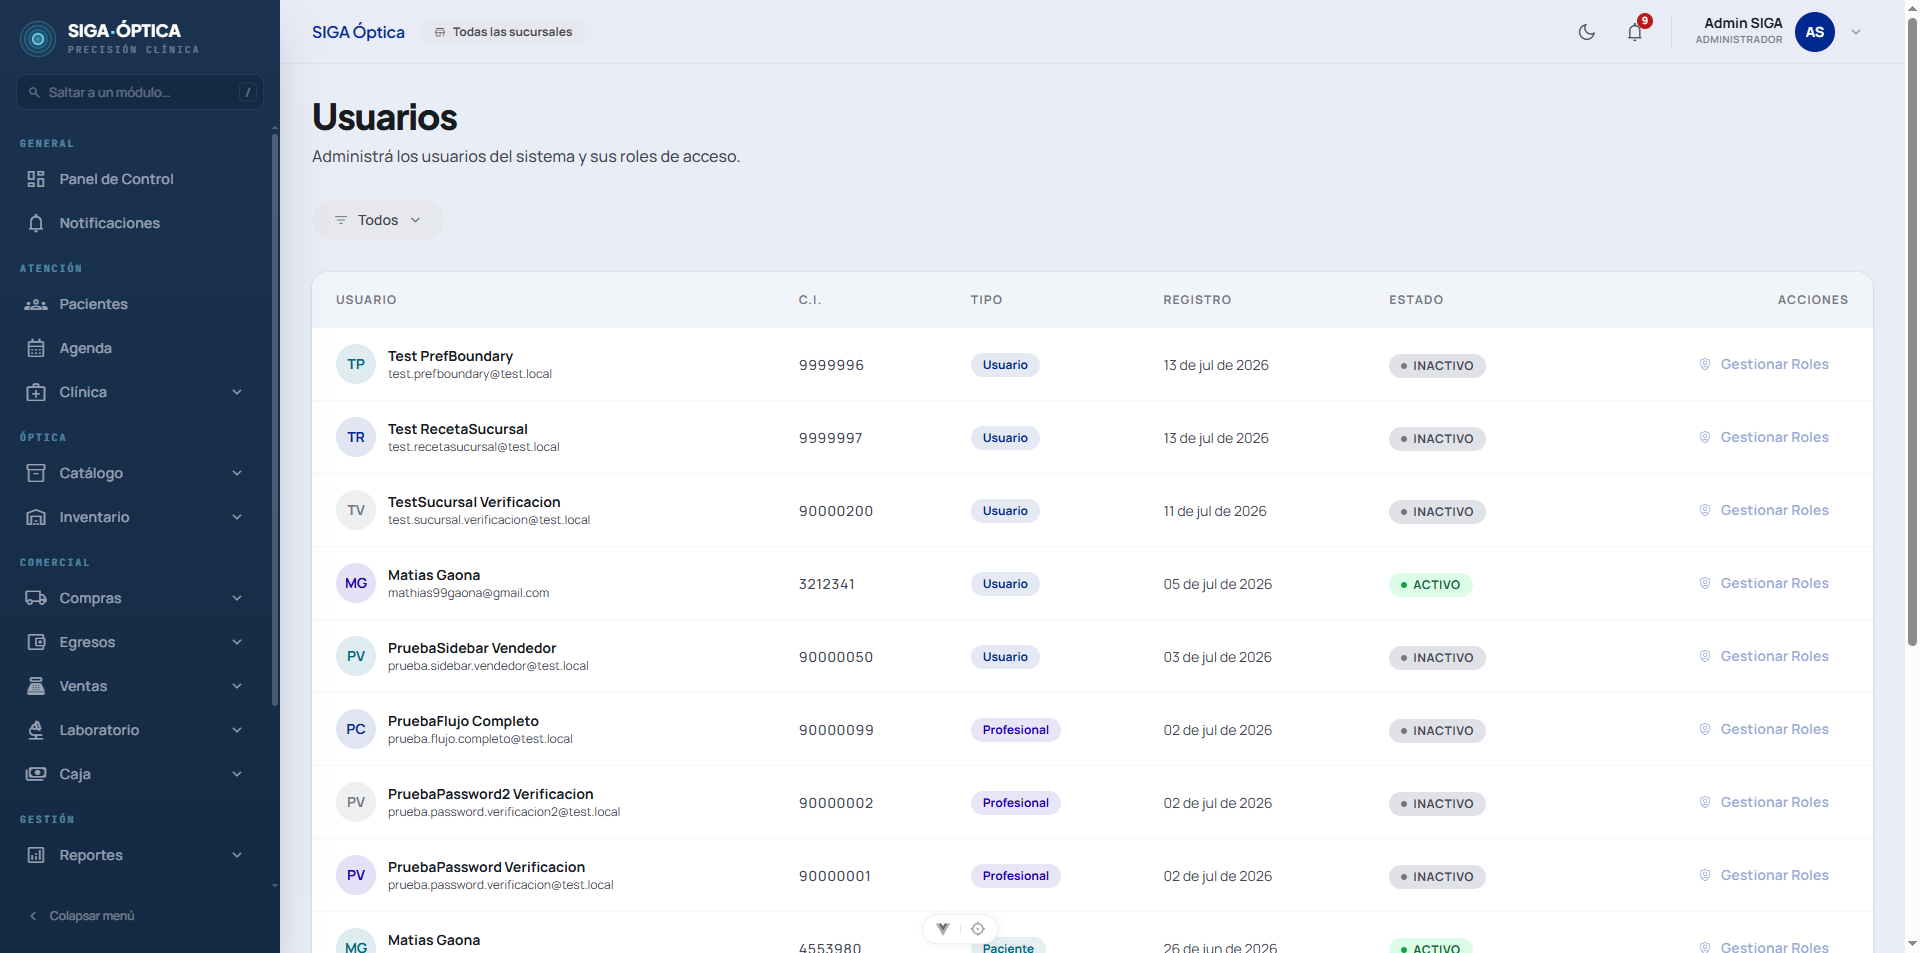
\includegraphics[width=0.8\textwidth]{imagenes/mod01-usuarios.png}
\caption{Sesión autenticada como administrador --- visibilidad completa de usuarios de ambas sucursales, sin la restricción que sí aplica a un usuario con sucursal fija.}
\label{fig:validacion-usuarios}
\end{figure}

\begin{figure}[htbp]
\centering
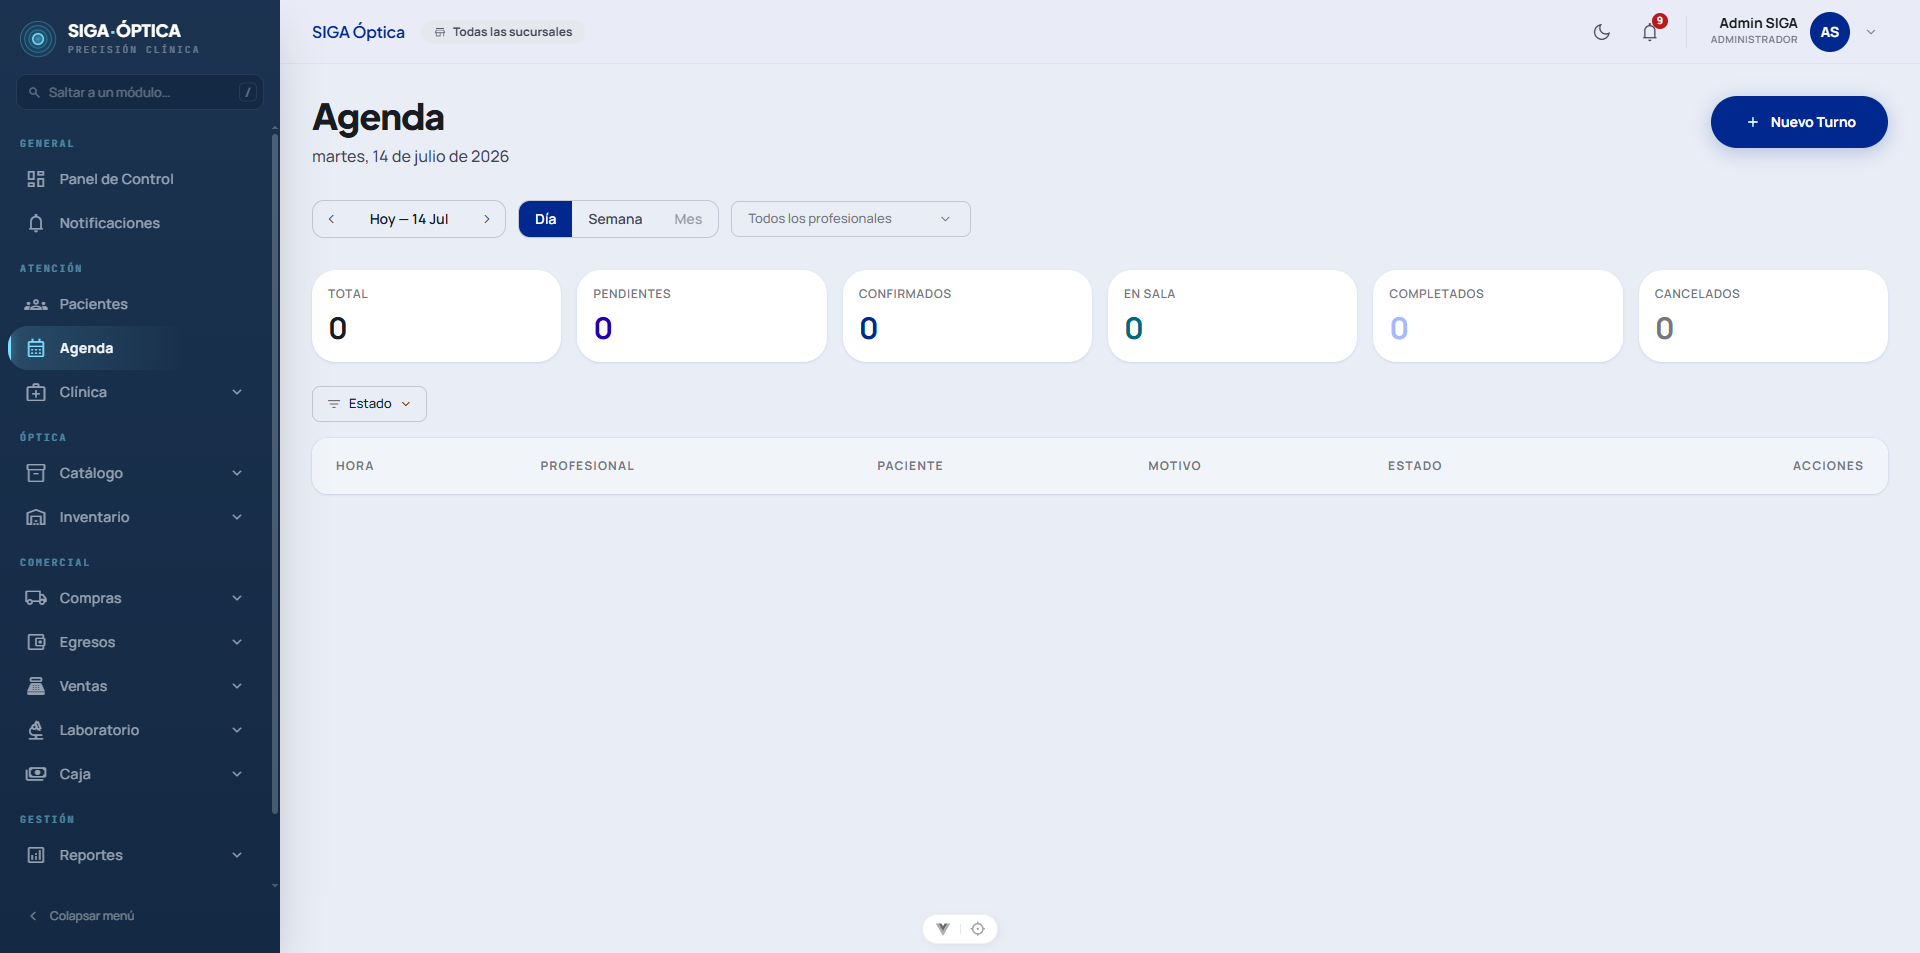
\includegraphics[width=0.8\textwidth]{imagenes/mod04-agenda.png}
\caption{Agenda de turnos verificada end-to-end: creación, confirmación y cancelación de citas.}
\label{fig:validacion-agenda}
\end{figure}

\begin{figure}[htbp]
\centering
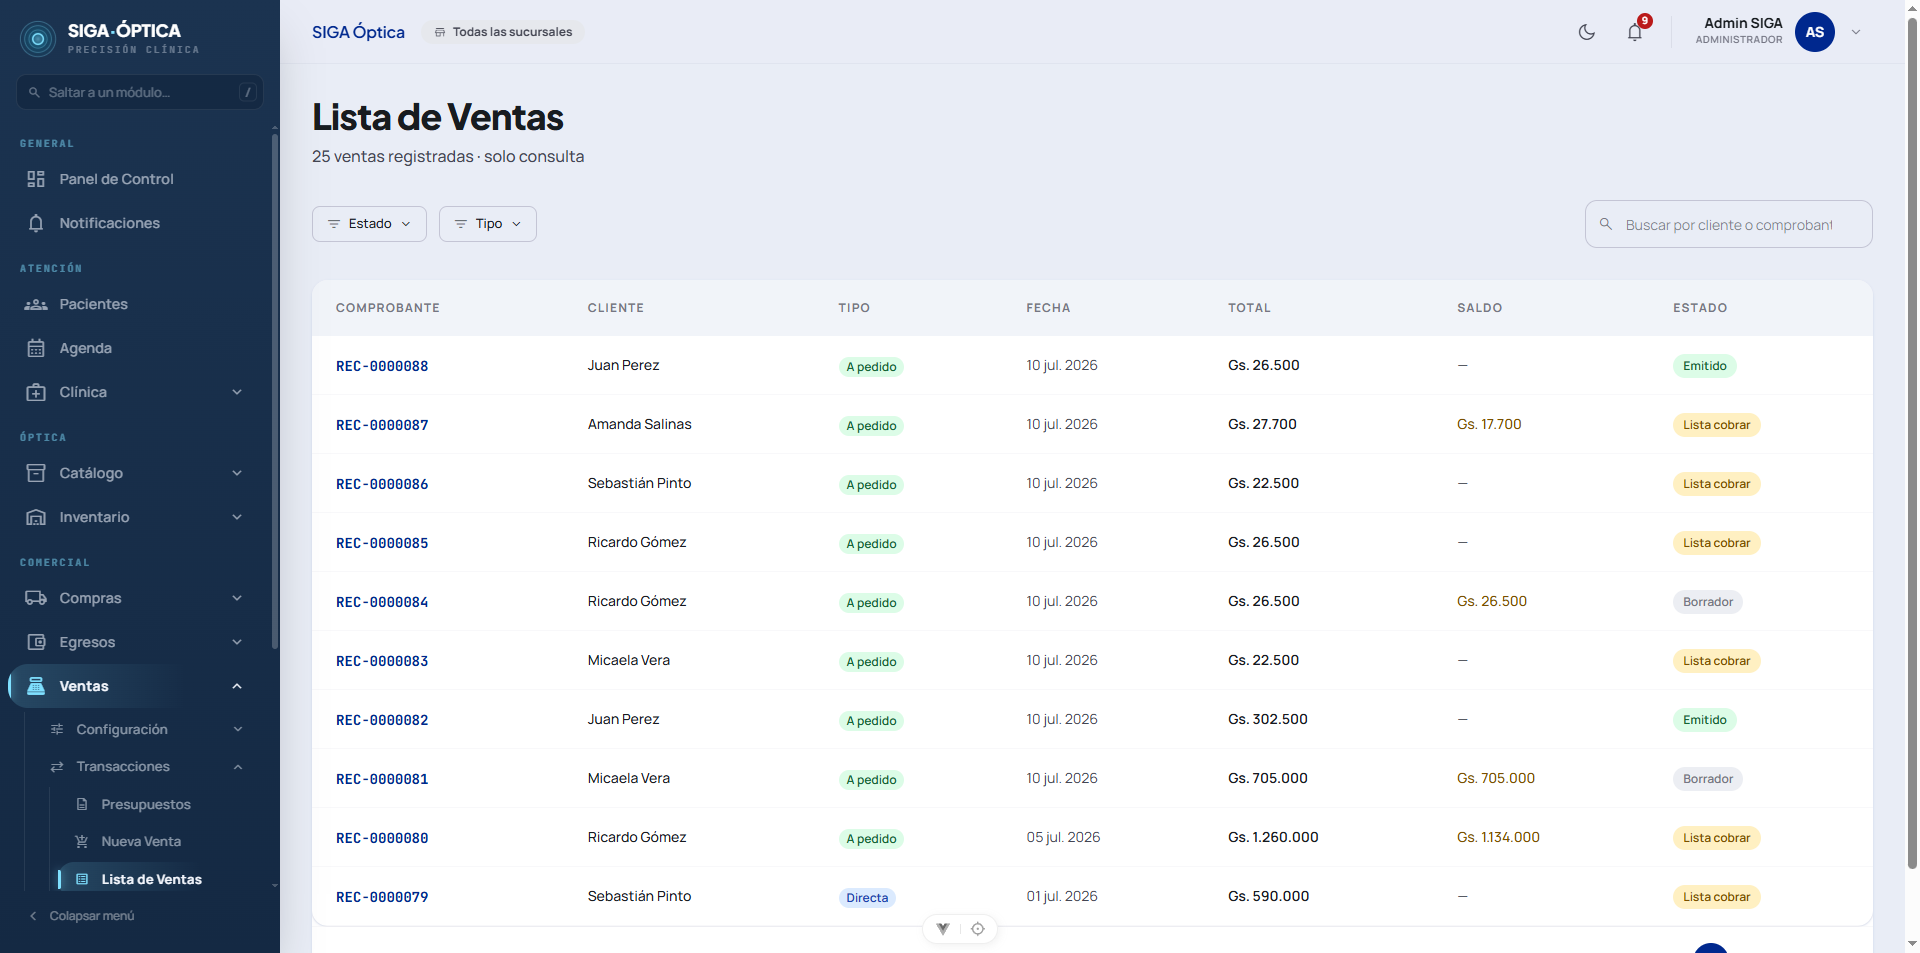
\includegraphics[width=0.8\textwidth]{imagenes/mod08-ventas.png}
\caption{Listado de ventas verificado tras ejercitar el ciclo completo de venta directa y venta a pedido, incluyendo presupuesto, confirmación, cobro y emisión de comprobante.}
\label{fig:validacion-ventas}
\end{figure}

\begin{figure}[htbp]
\centering
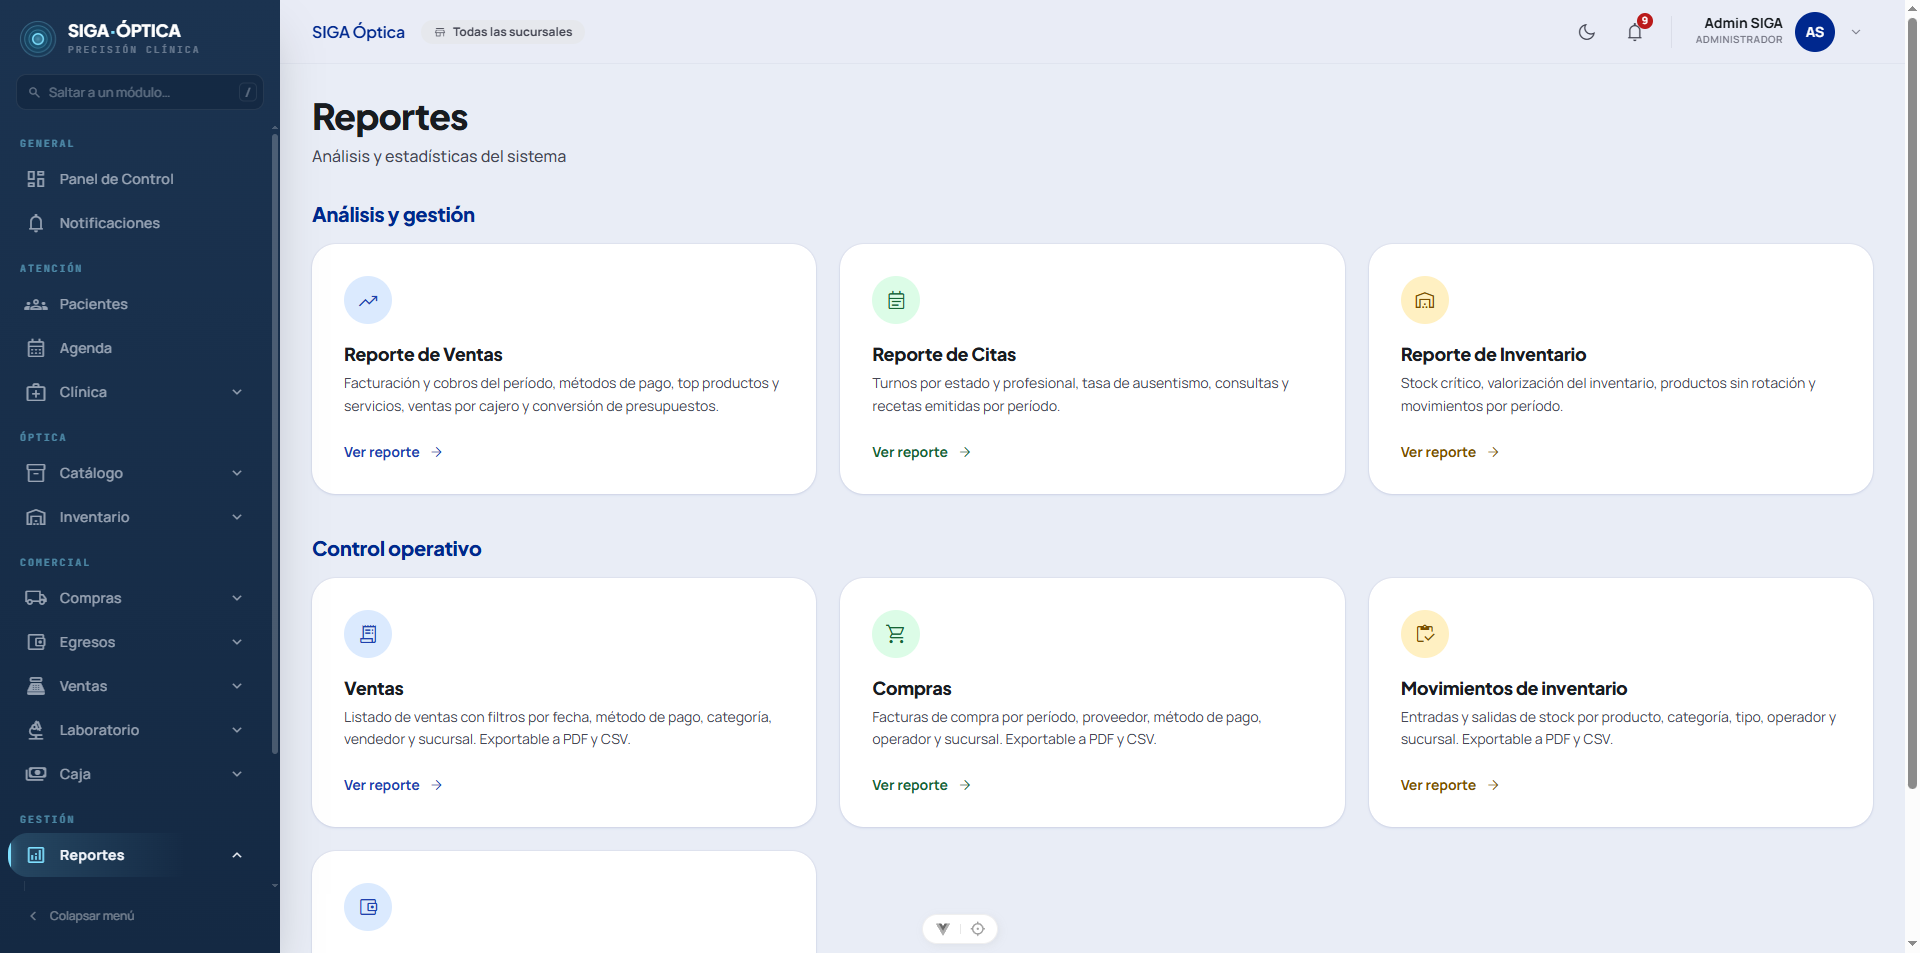
\includegraphics[width=0.8\textwidth]{imagenes/mod14-reportes.png}
\caption{Panel de reportes desde el cual se ejercitaron las ocho combinaciones de exportación (cuatro reportes operativos por dos formatos) descriptas en la Sección~\ref{sec:validacion-reportes}.}
\label{fig:validacion-reportes}
\end{figure}
